% ---------------------------------------------------------------------------
% Author guideline and sample document for EG publication using LaTeX2e input
% D.Fellner, v1.12, Nov 01, 2006

\documentclass[]{egpubl}
\usepackage{eg-it2015}

% --- for  Annual CONFERENCE
% \ConferenceSubmission % uncomment for Conference submission
% \ConferencePaper      % uncomment for (final) Conference Paper
% \STAR                 % uncomment for STAR contribution
% \Tutorial             % uncomment for Tutorial contribution
% \ShortPresentation    % uncomment for (final) Short Conference Presentation
%
% --- for  CGF Journal
% \JournalSubmission    % uncomment for submission to Computer Graphics Forum
% \JournalPaper         % uncomment for final version of Journal Paper
%
% --- for  EG Workshop Proceedings
% \WsSubmission    % uncomment for submission to EG Workshop
 \WsPaper         % uncomment for final version of EG Workshop contribution
%
 \electronicVersion % can be used both for the printed and electronic version

% !! *please* don't change anything above
% !! unless you REALLY know what you are doing
% ------------------------------------------------------------------------

% for including postscript figures
% mind: package option 'draft' will replace PS figure by a filename within a frame
\ifpdf \usepackage[pdftex]{graphicx} \pdfcompresslevel=9
\else \usepackage[dvips]{graphicx} \fi

\PrintedOrElectronic

% prepare for electronic version of your document
\usepackage{t1enc,dfadobe}

\usepackage{egweblnk}
\usepackage{cite}

% For backwards compatibility to old LaTeX type font selection.
% Uncomment if your document adheres to LaTeX2e recommendations.
% \let\rm=\rmfamily    \let\sf=\sffamily    \let\tt=\ttfamily
% \let\it=\itshape     \let\sl=\slshape     \let\sc=\scshape
% \let\bf=\bfseries

% end of prologue


\nonstopmode
% ------------------------------------------------------------------------

% if the Editors-in-Chief have given you the data, you may uncomment
% the following five lines and insert it here
%
% \volume{27}   % the volume in which the issue will be published;
% \issue{1}     % the issue number of the publication
% \pStartPage{1}      % set starting page



\usepackage{balance}

\usepackage{graphicx}
\usepackage{caption}
\usepackage{subcaption}
\usepackage{hyperref}

\usepackage{listings}
\usepackage{xcolor}


\colorlet{punct}{red!60!black}
\definecolor{background}{HTML}{FEFEFE}
\definecolor{delim}{RGB}{20,105,176}
\colorlet{numb}{magenta!60!black}

\lstdefinelanguage{json}{
    basicstyle=\small\ttfamily,
    % numbers=left,
    % numberstyle=\scriptsize,
    % stepnumber=1,
    % numbersep=8pt,
    % showstringspaces=false,
    % breaklines=true,
    % frame=lines,
    backgroundcolor=\color{background},
    literate=
     *{0}{{{\color{numb}0}}}{1}
      {1}{{{\color{numb}1}}}{1}
      {2}{{{\color{numb}2}}}{1}
      {3}{{{\color{numb}3}}}{1}
      {4}{{{\color{numb}4}}}{1}
      {5}{{{\color{numb}5}}}{1}
      {6}{{{\color{numb}6}}}{1}
      {7}{{{\color{numb}7}}}{1}
      {8}{{{\color{numb}8}}}{1}
      {9}{{{\color{numb}9}}}{1}
      {:}{{{\color{punct}{:}}}}{1}
      {,}{{{\color{punct}{,}}}}{1}
      {\{}{{{\color{delim}{\{}}}}{1}
      {\}}{{{\color{delim}{\}}}}}{1}
      {[}{{{\color{delim}{[}}}}{1}
      {]}{{{\color{delim}{]}}}}{1},
}

%----macros begin---------------------------------------------------------------
\usepackage{amssymb}
\usepackage{color}

\def\conv{\mbox{\textrm{conv}\,}}
\def\aff{\mbox{\textrm{aff}\,}}
\def\E{\mathbb{E}}
\def\R{\mathbb{R}}
\def\Z{\mathbb{Z}}
\def\tex{\TeX}
\def\latex{\LaTeX}
\def\v#1{{\bf #1}}
\def\p#1{{\bf #1}}
\def\T#1{{\bf #1}}

\def\vet#1{{\left(\begin{array}{cccccccccccccccccccc}#1\end{array}\right)}}
\def\mat#1{{\left(\begin{array}{cccccccccccccccccccc}#1\end{array}\right)}}

\def\lin{\mbox{\rm lin}\,}
\def\aff{\mbox{\rm aff}\,}
\def\pos{\mbox{\rm pos}\,}
\def\cone{\mbox{\rm cone}\,}
\def\conv{\mbox{\rm conv}\,}
\newcommand{\homog}[0]{\mbox{\rm homog}\,}
\newcommand{\relint}[0]{\mbox{\rm relint}\,}

%----macros end-----------------------------------------------------------------
\begin{document}


\begin{figure*}[htbp] %  figure placement: here, top, bottom, or page
   \centering
\hspace{-3mm}   
   \begin{subfigure}[b]{0.175\textwidth}
   
\includegraphics[width=\textwidth]{images/zigzag1}
   \caption{}
   \end{subfigure}
~
   \begin{subfigure}[b]{0.175\textwidth}
   
\includegraphics[width=\textwidth]{images/zigzag2}
   \caption{}
   \end{subfigure}
~
   \begin{subfigure}[b]{0.175\textwidth}
   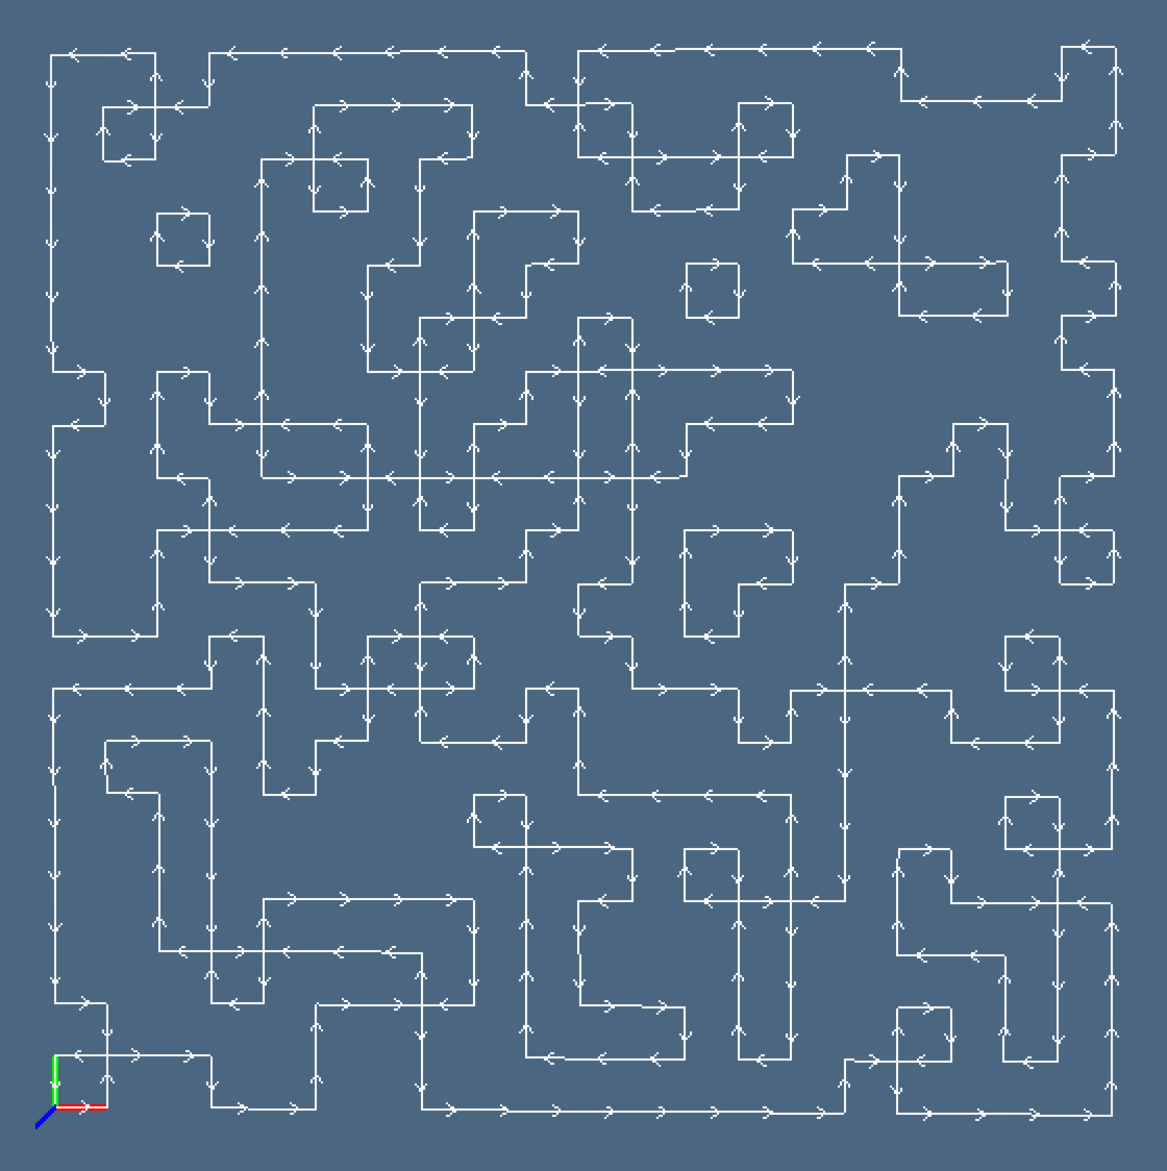
\includegraphics[width=\textwidth]{images/zigzag3}
   \caption{}
   \end{subfigure}
~
   \begin{subfigure}[b]{0.175\textwidth}
   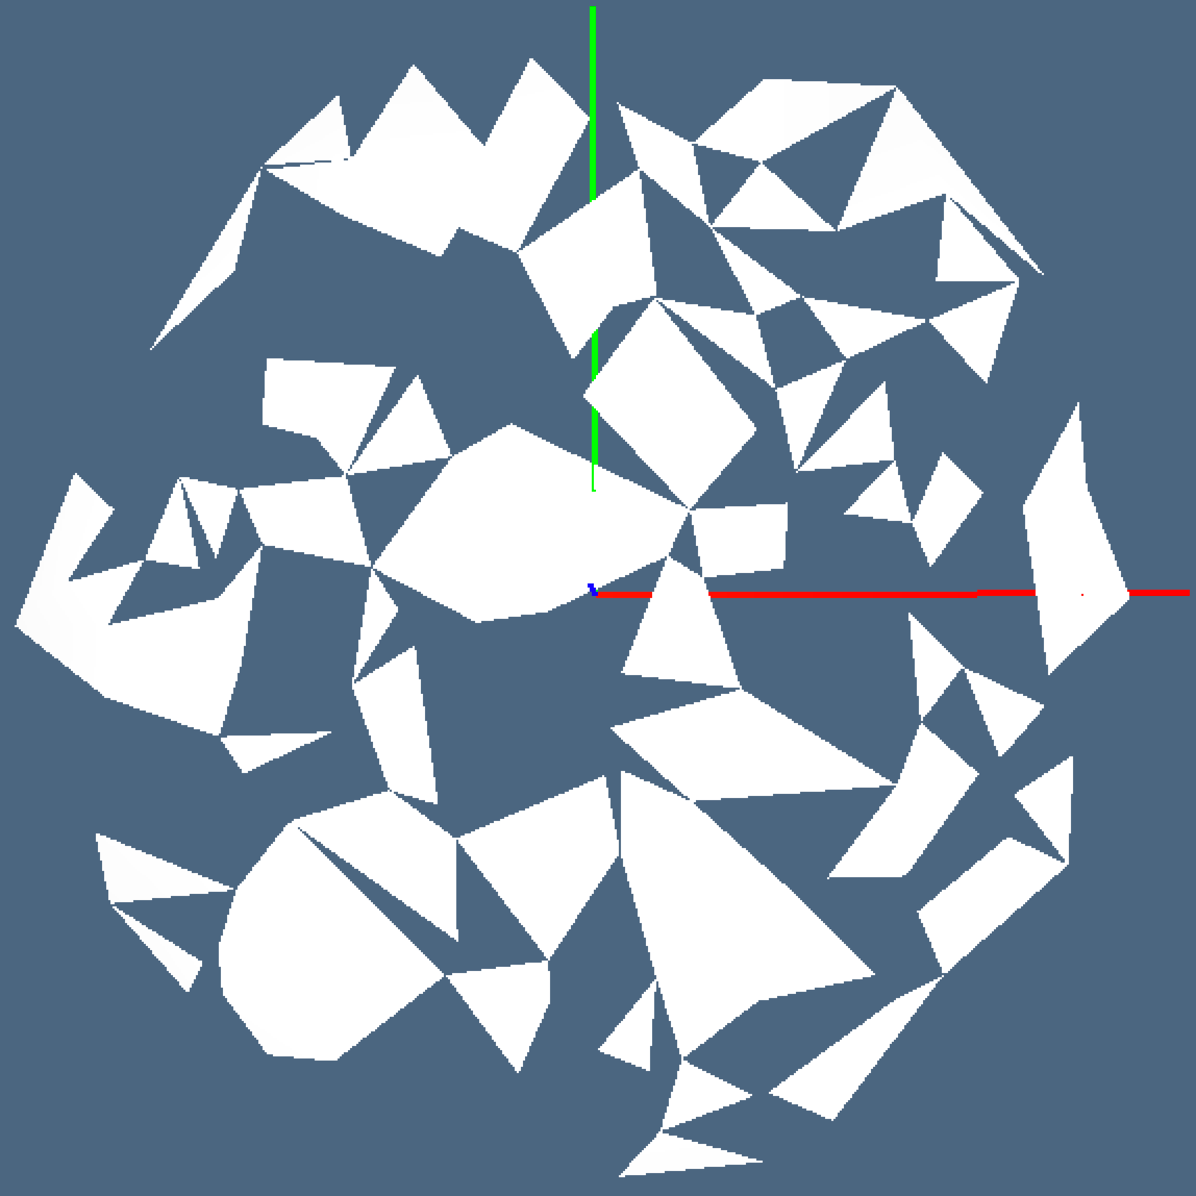
\includegraphics[width=\textwidth]{images/randomdelaunay1}
   \caption{}
   \end{subfigure}
~
   \begin{subfigure}[b]{0.175\textwidth}
   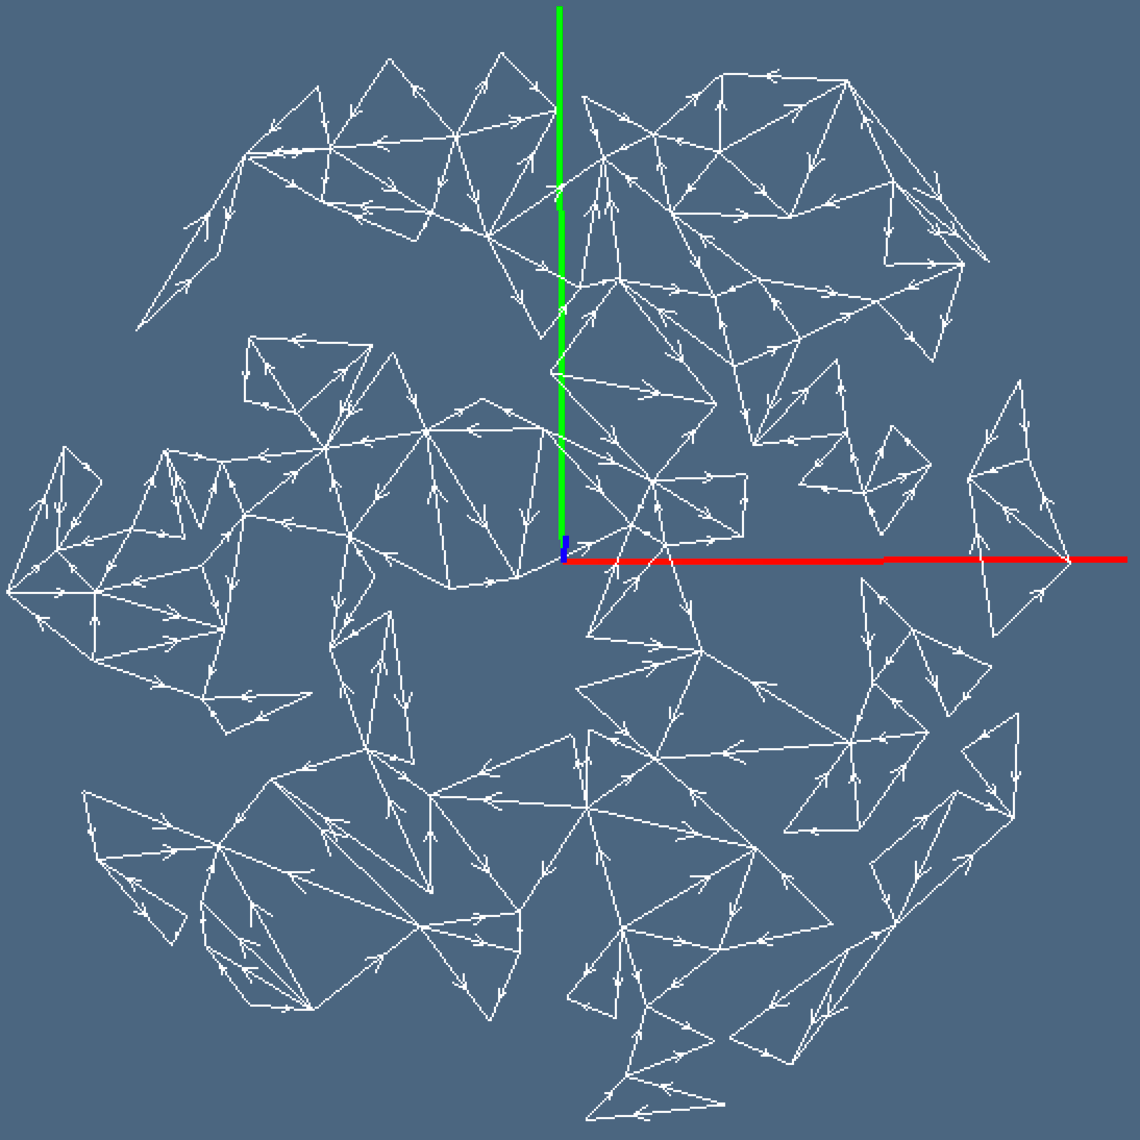
\includegraphics[width=\textwidth]{images/randomdelaunay2}
   \caption{}
   \end{subfigure}
~
   \begin{subfigure}[b]{0.175\textwidth}
   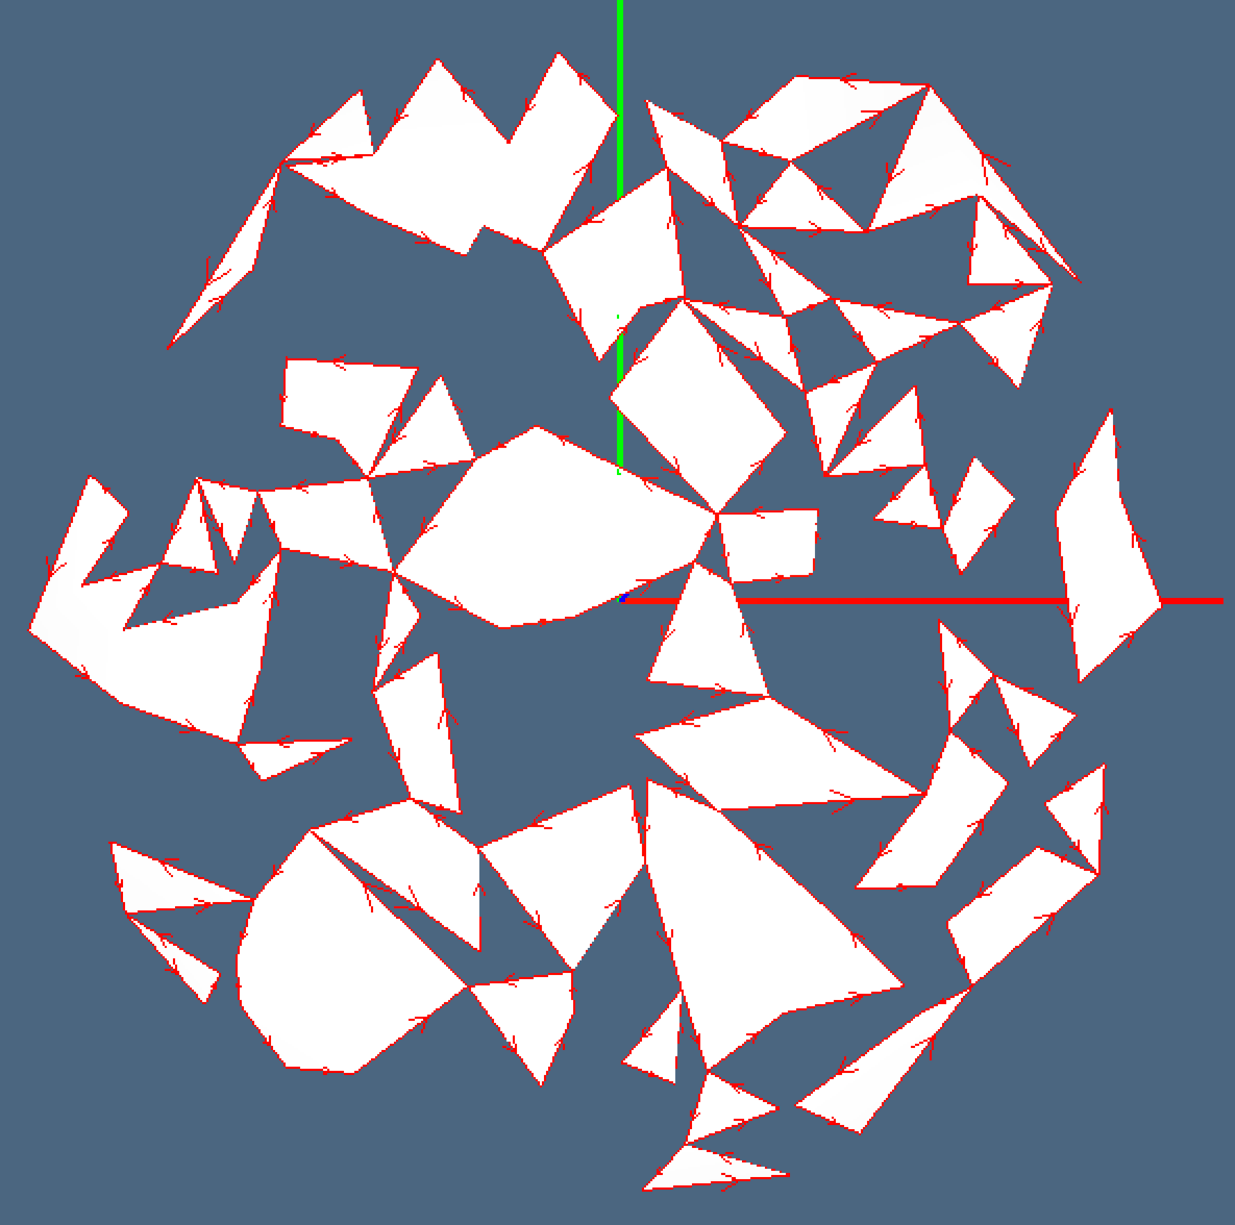
\includegraphics[width=\textwidth]{images/randomdelaunay3}
   \caption{}
   \end{subfigure}
   
   \caption{LAR examples: (a) 2-chain of quad cells; (b) boundary 1-chain; (c) oriented boundary; (d) random 2-complex; (e) oriented 1-skeleton; (f) oriented boundary (in red).}
   \label{fig:meshes}
\end{figure*}


\begin{figure*}[htbp] %  figure placement: here, top, bottom, or page
   \centering
\hspace{-3mm}   
   \begin{subfigure}[b]{0.175\textwidth}
   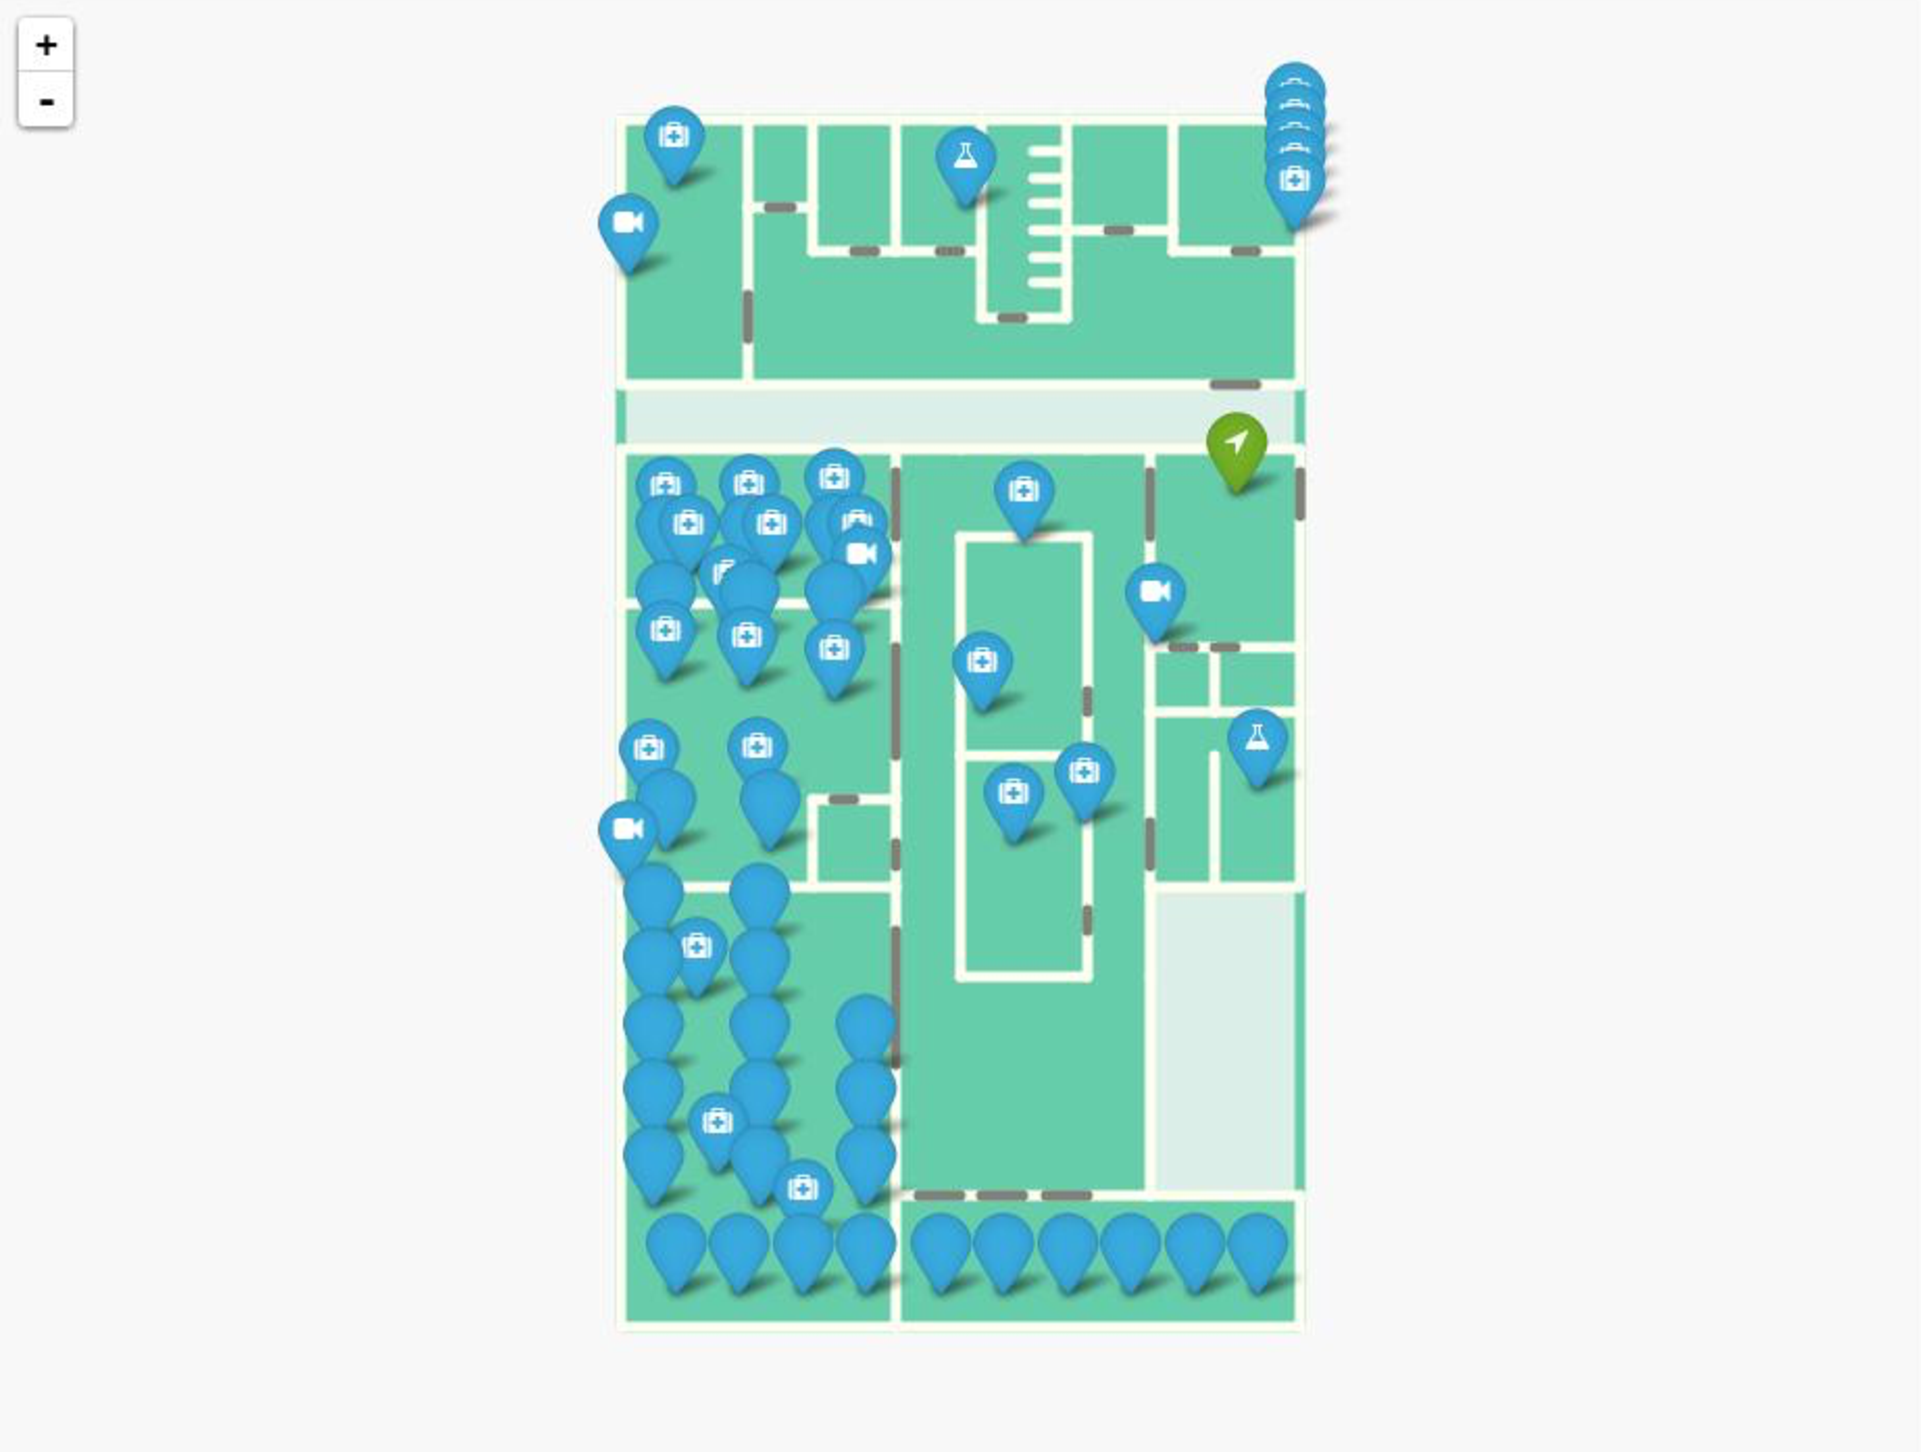
\includegraphics[width=\textwidth]{images/emergency/13}
   \caption{}
   \end{subfigure}
\hspace{-3mm}   
   \begin{subfigure}[b]{0.175\textwidth}
   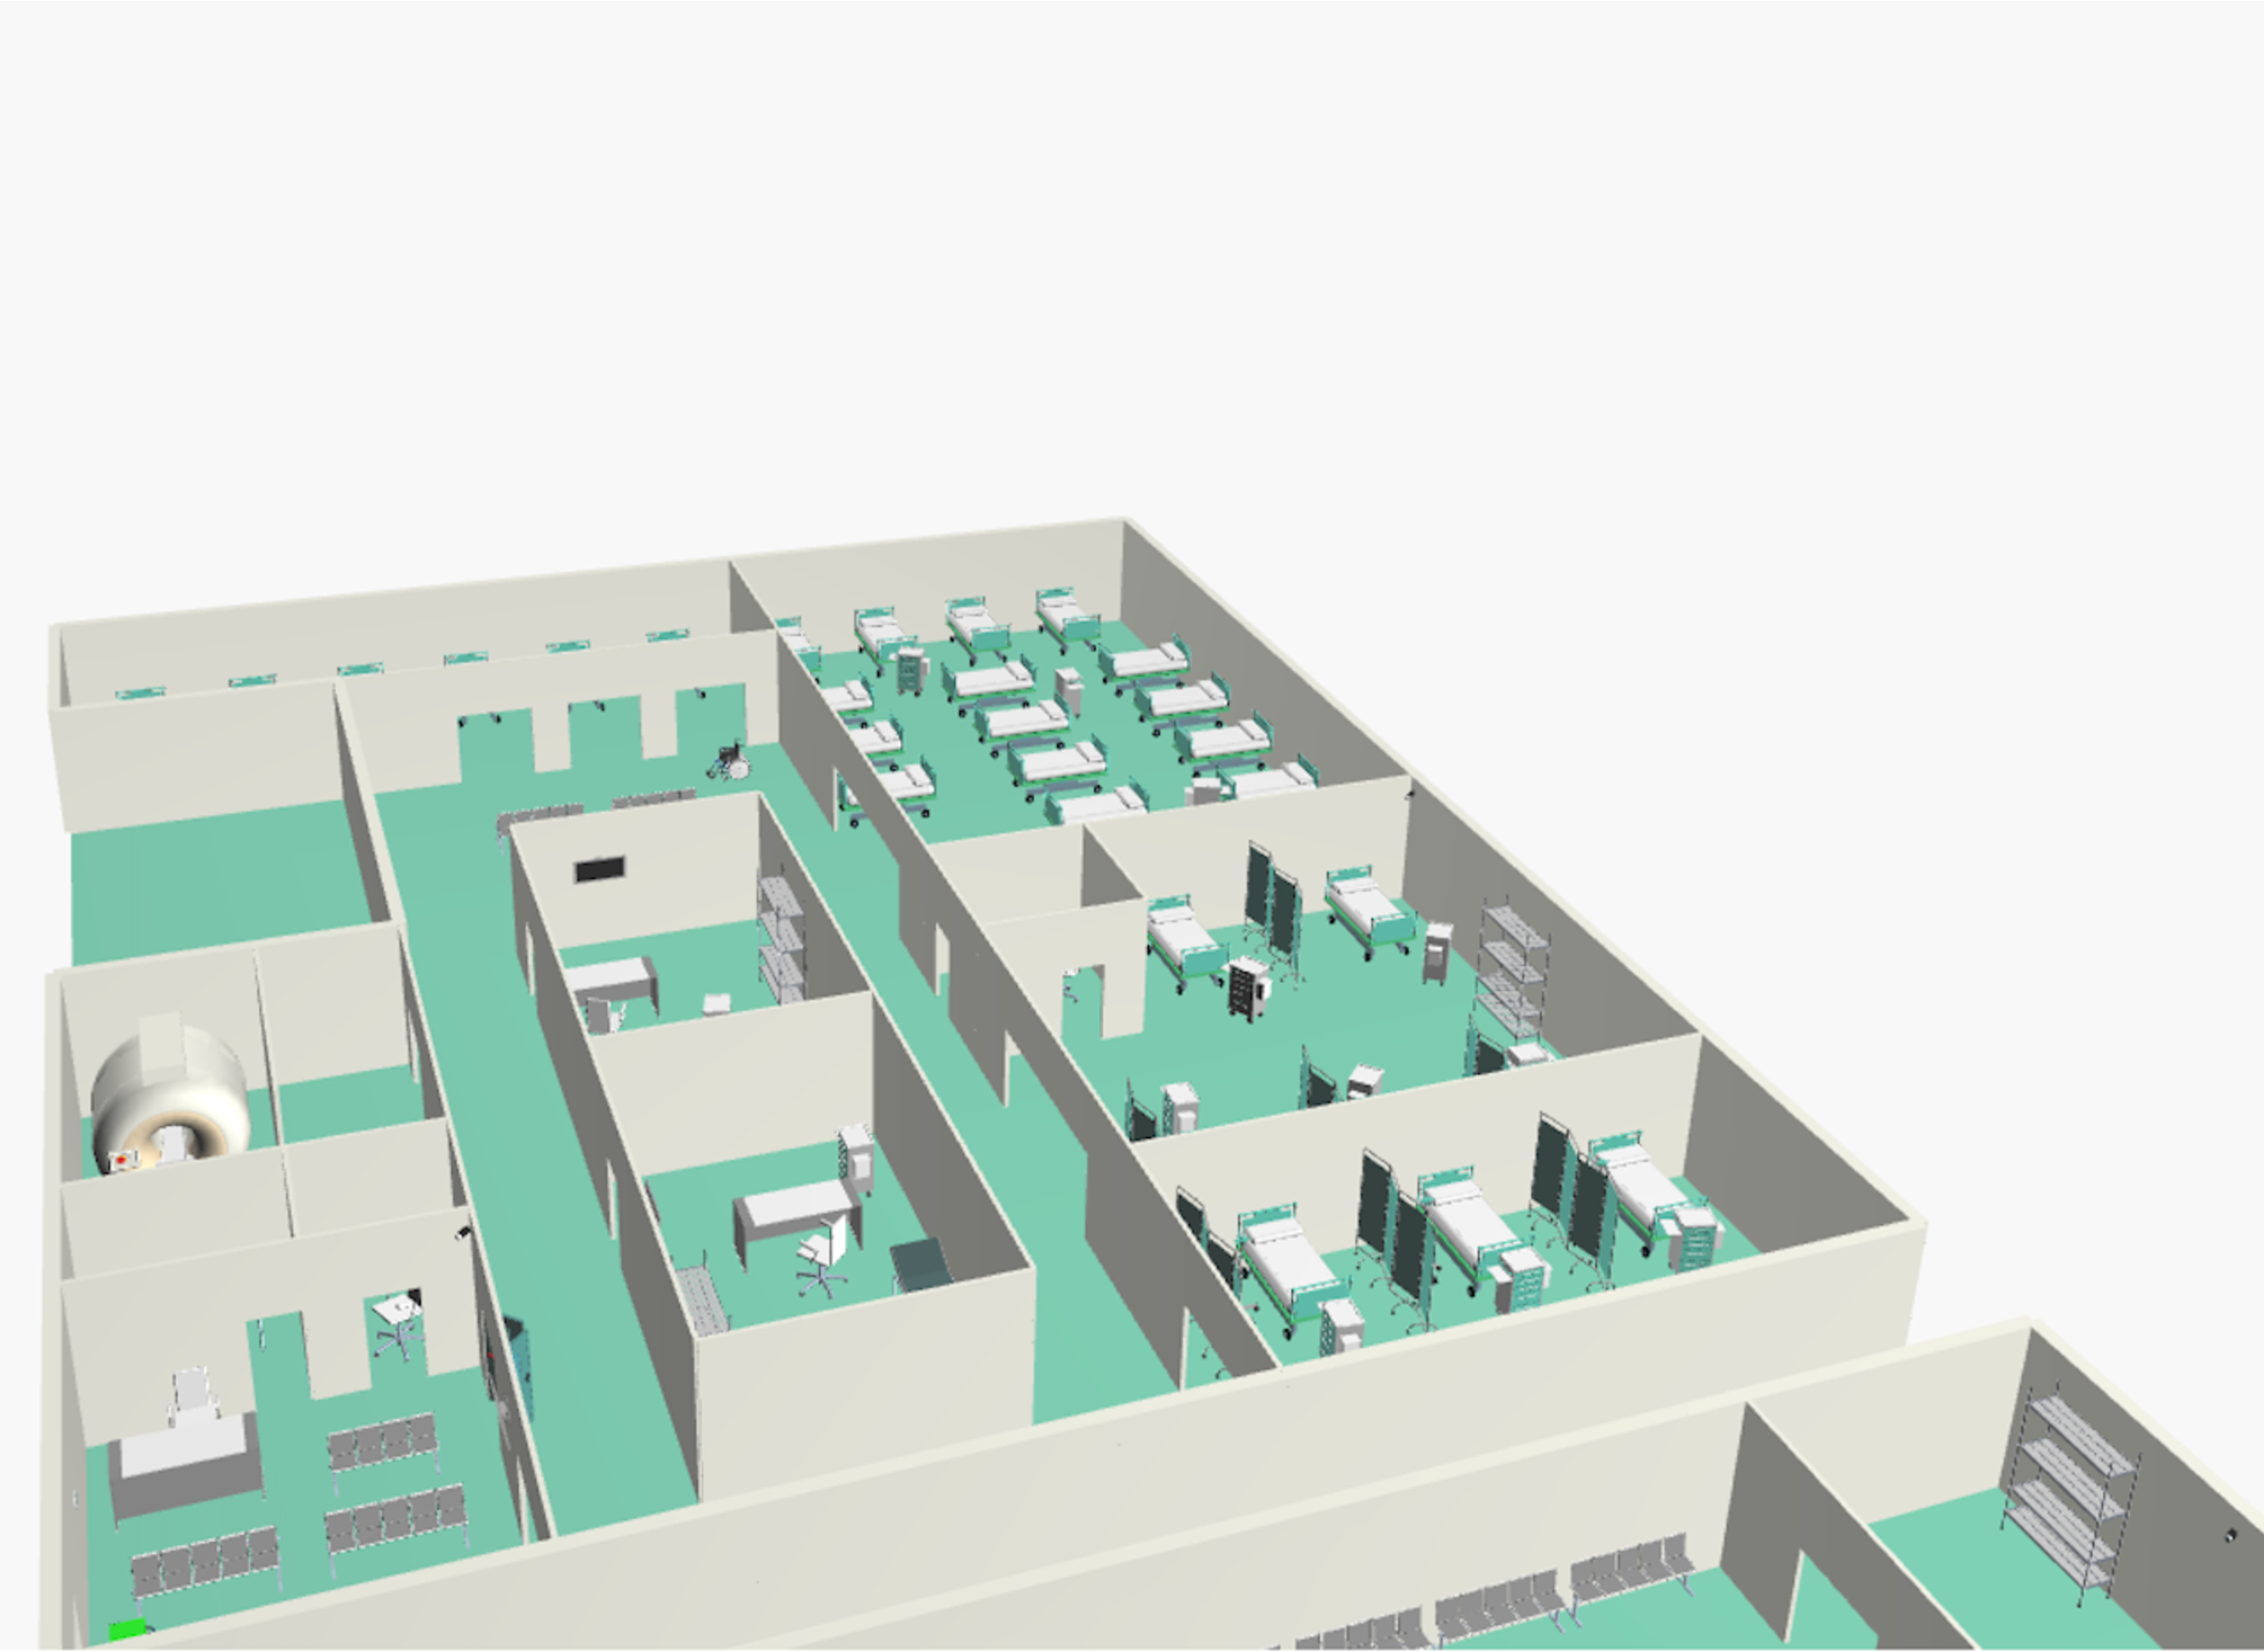
\includegraphics[width=\textwidth]{images/emergency/14}
   \caption{}
   \end{subfigure}
\hspace{-3mm}   
   \begin{subfigure}[b]{0.175\textwidth}
   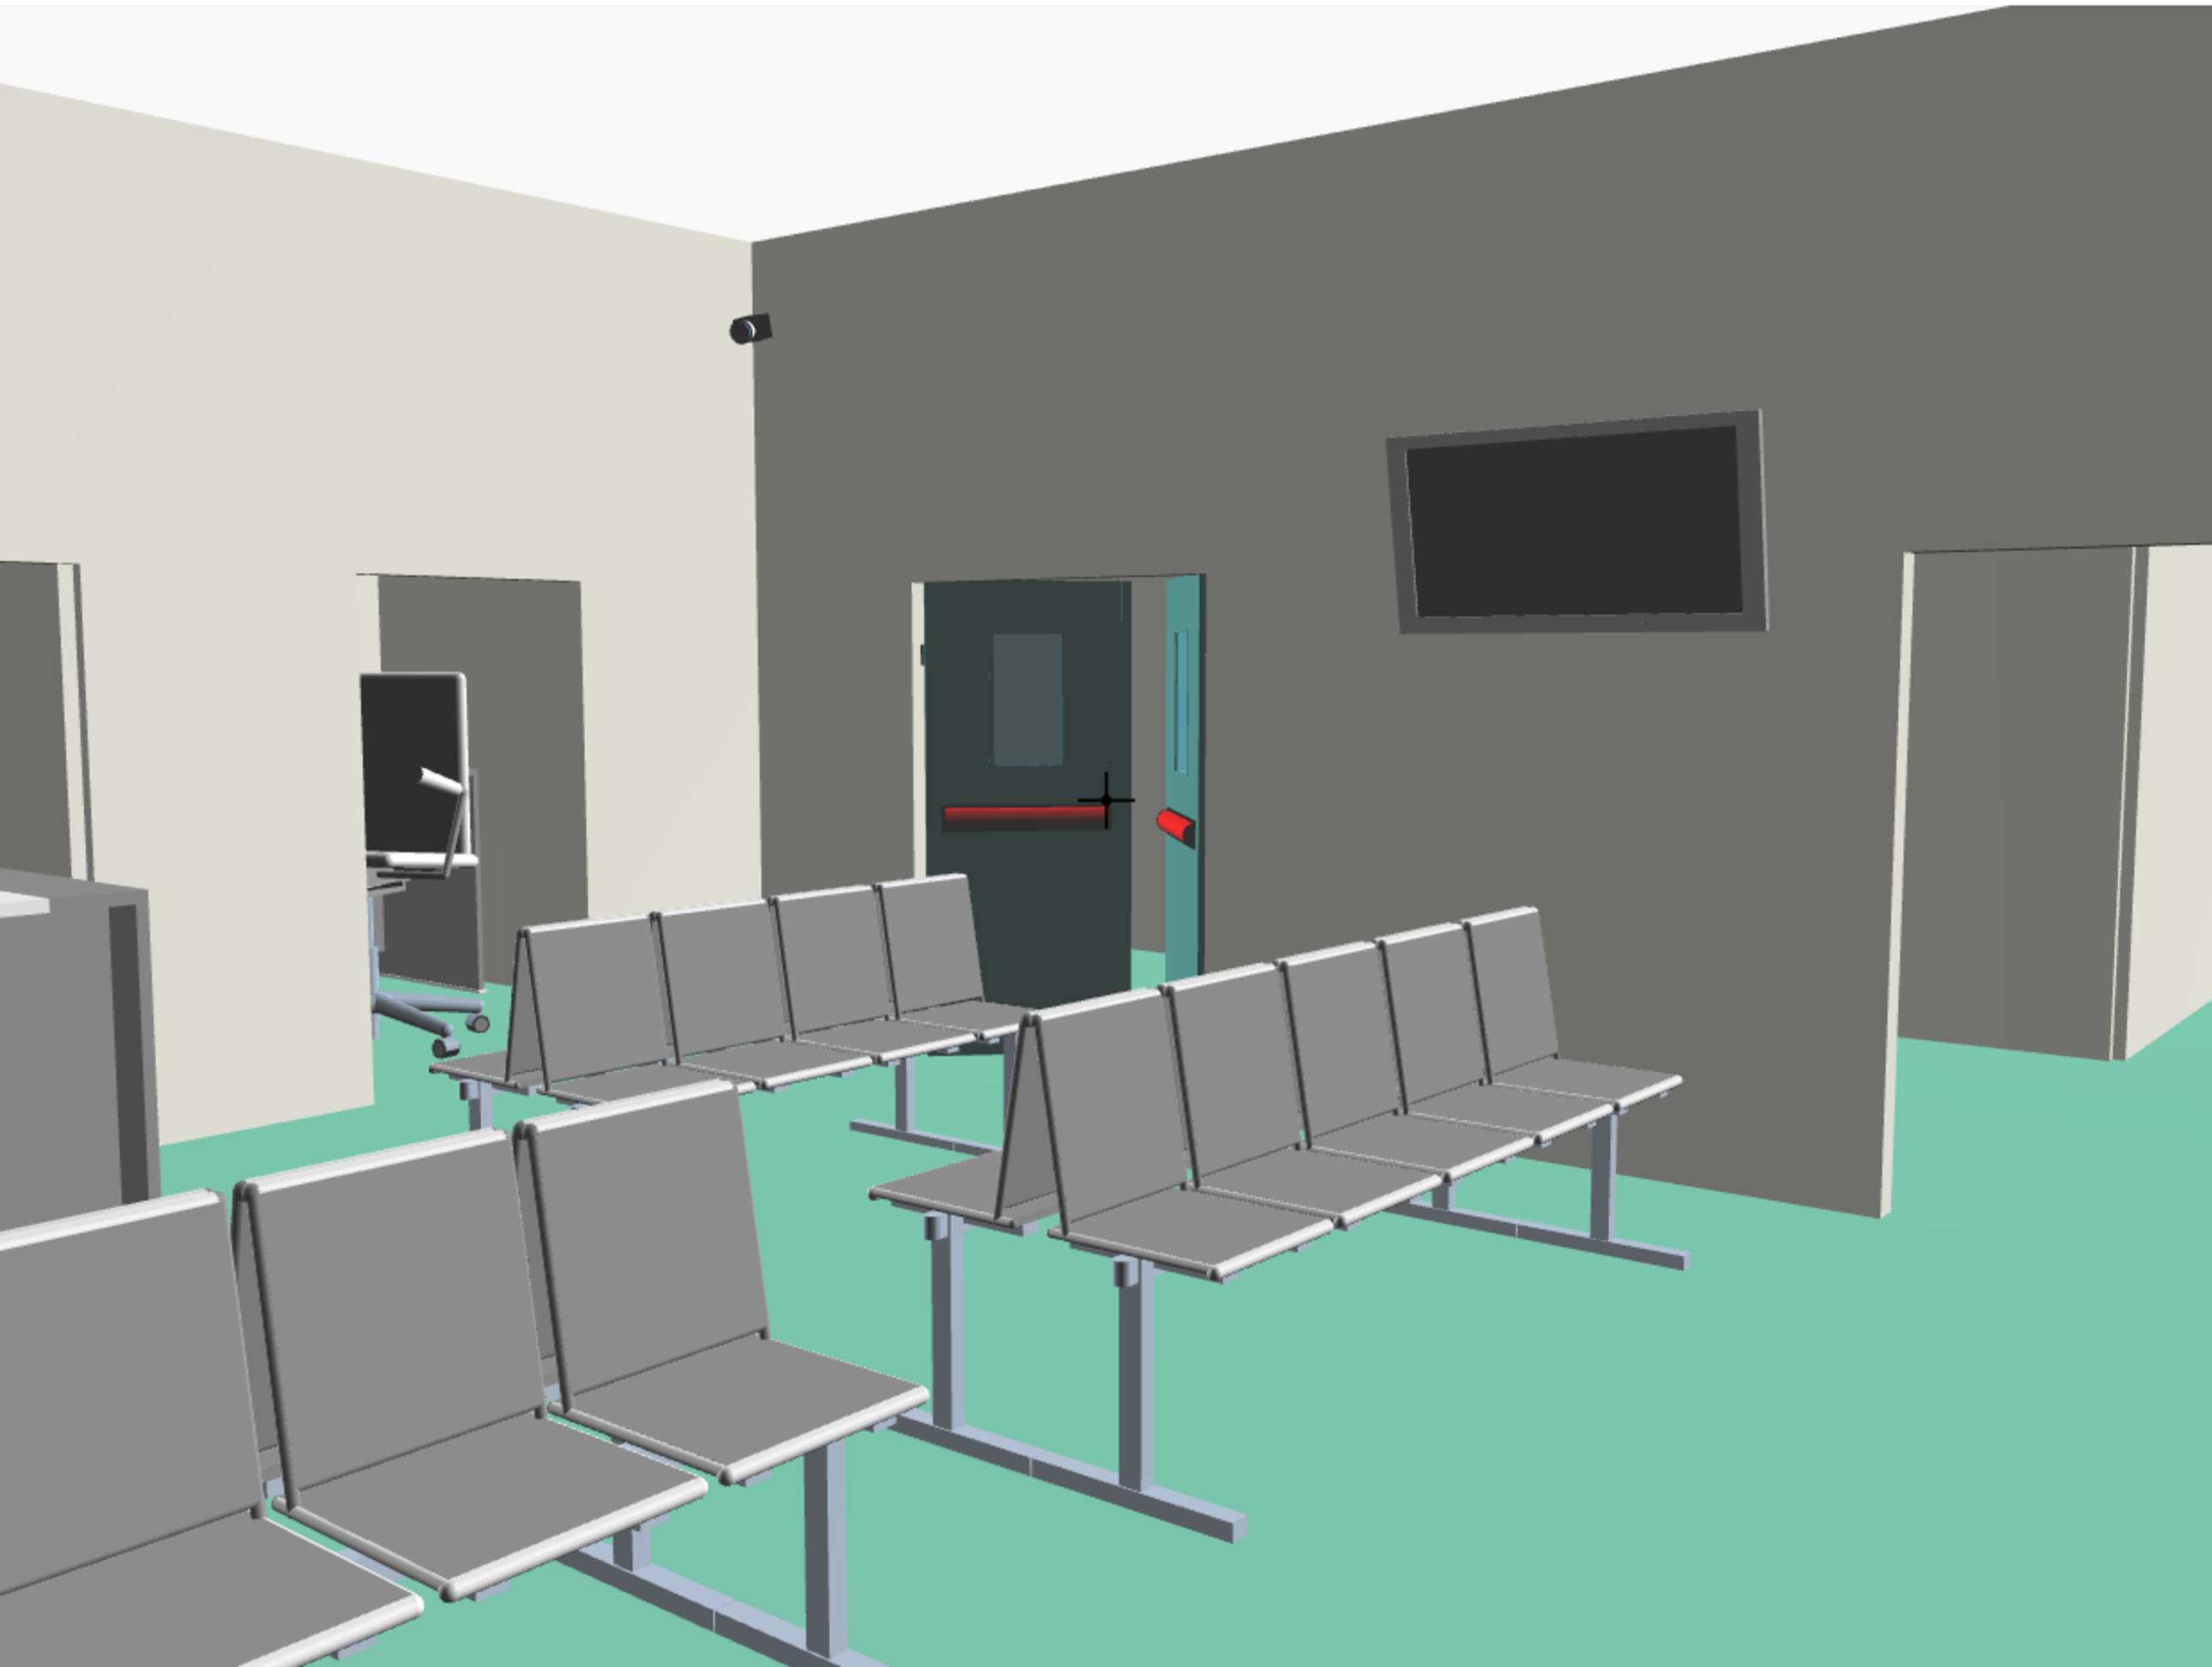
\includegraphics[width=\textwidth]{images/emergency/4}
   \caption{}
   \end{subfigure}
\hspace{-3mm}   
   \begin{subfigure}[b]{0.175\textwidth}
   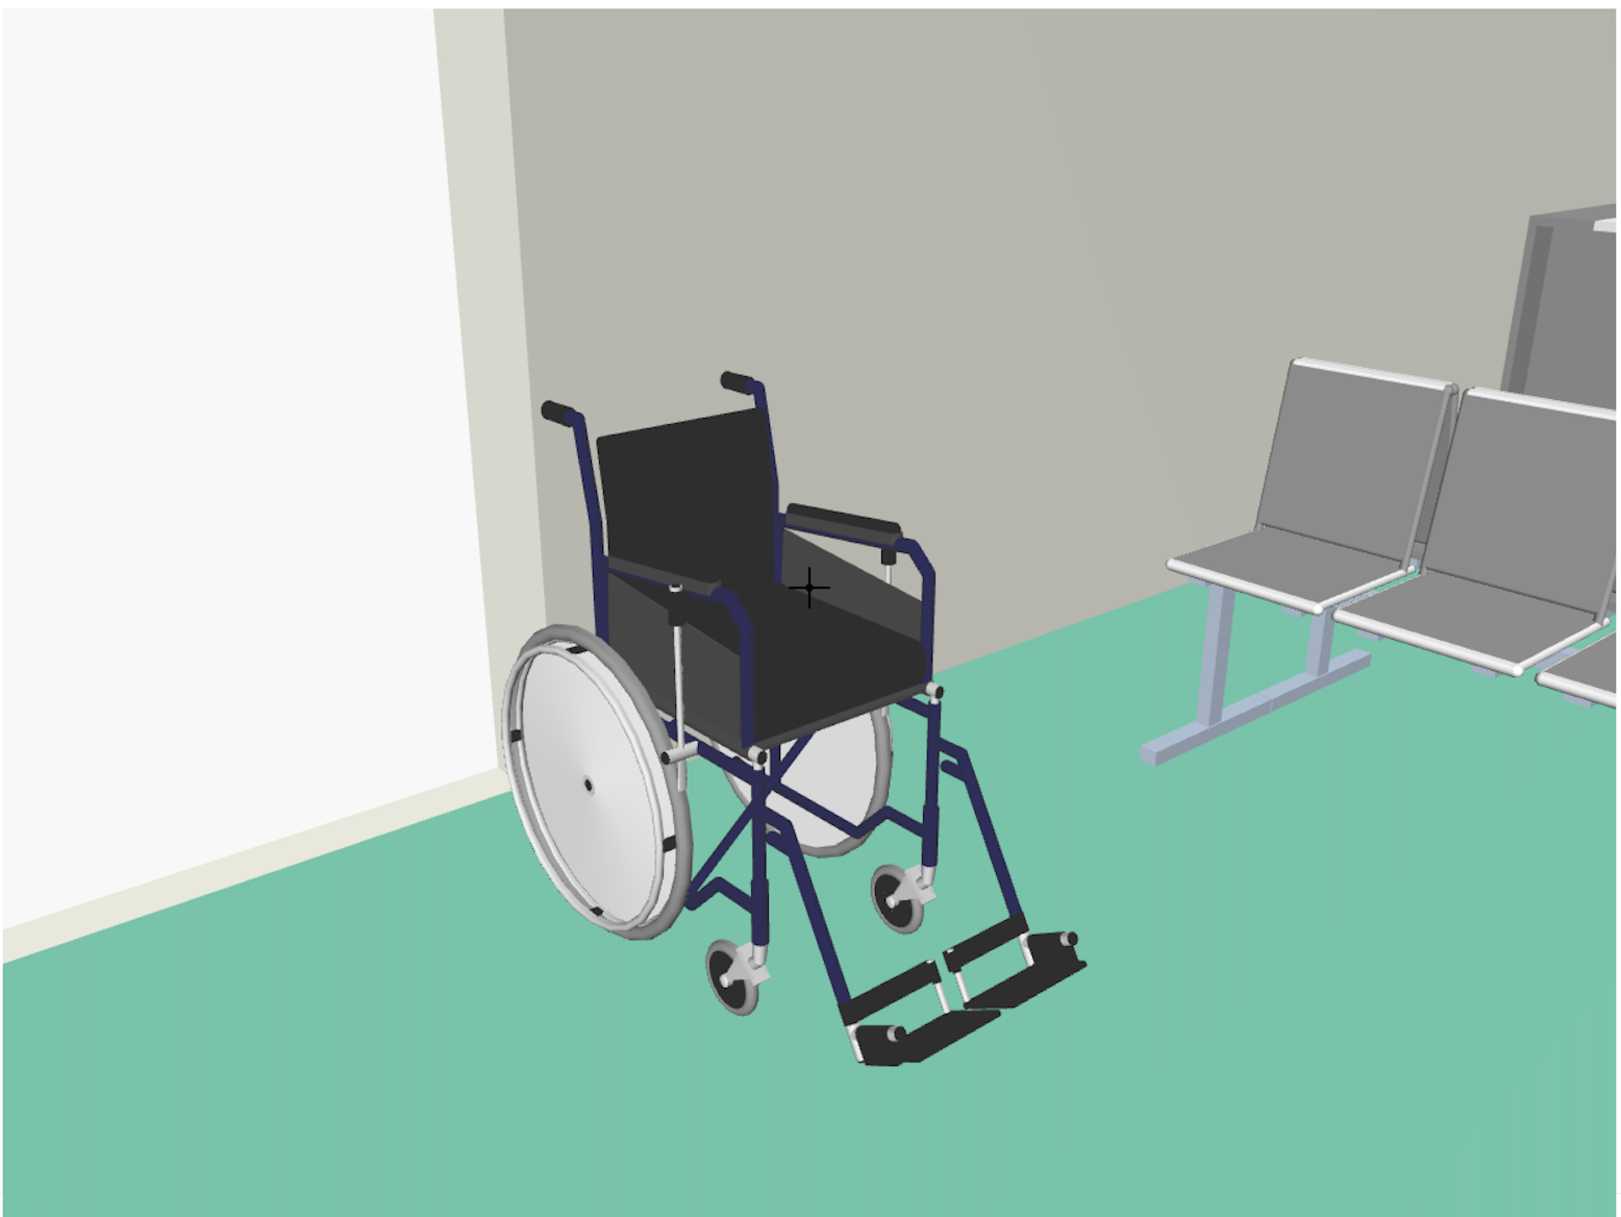
\includegraphics[width=\textwidth]{images/emergency/5}
   \caption{}
   \end{subfigure}
\hspace{-3mm}   
   \begin{subfigure}[b]{0.175\textwidth}
   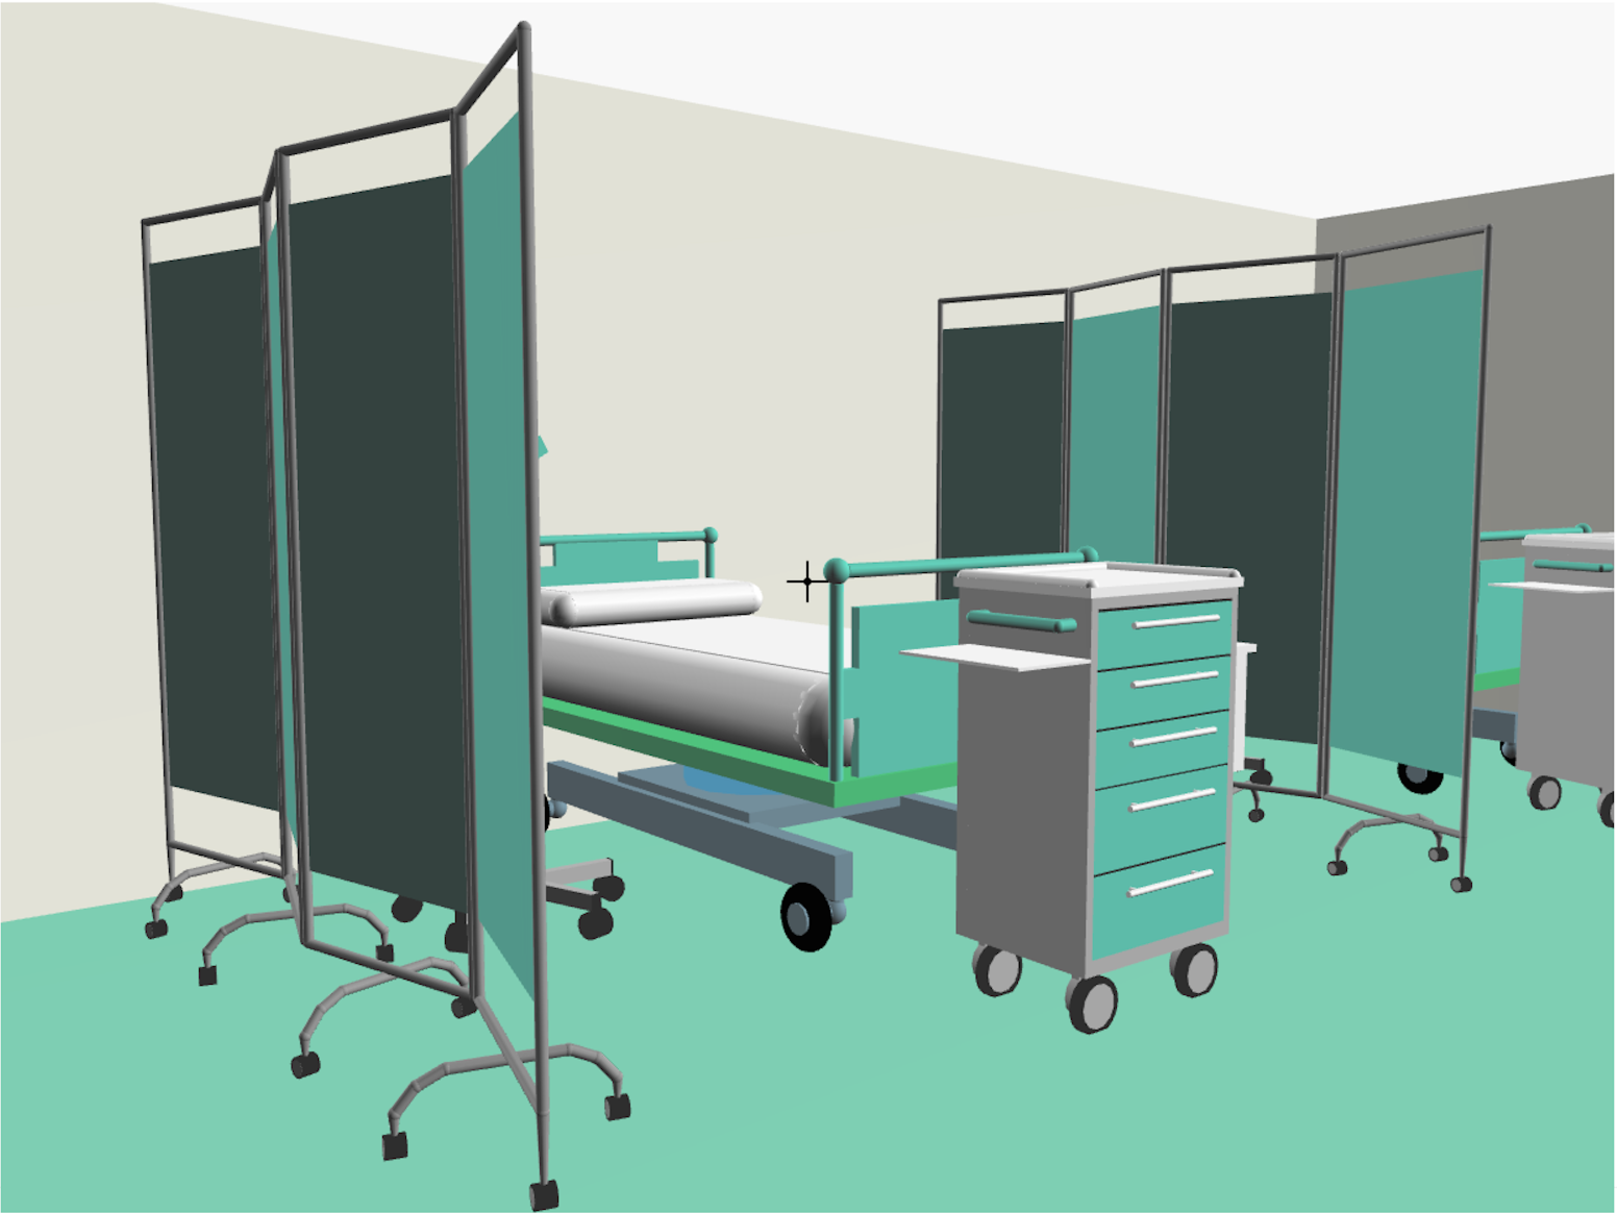
\includegraphics[width=\textwidth]{images/emergency/6}
   \caption{}
   \end{subfigure}
\hspace{-3mm}   
   \begin{subfigure}[b]{0.175\textwidth}
   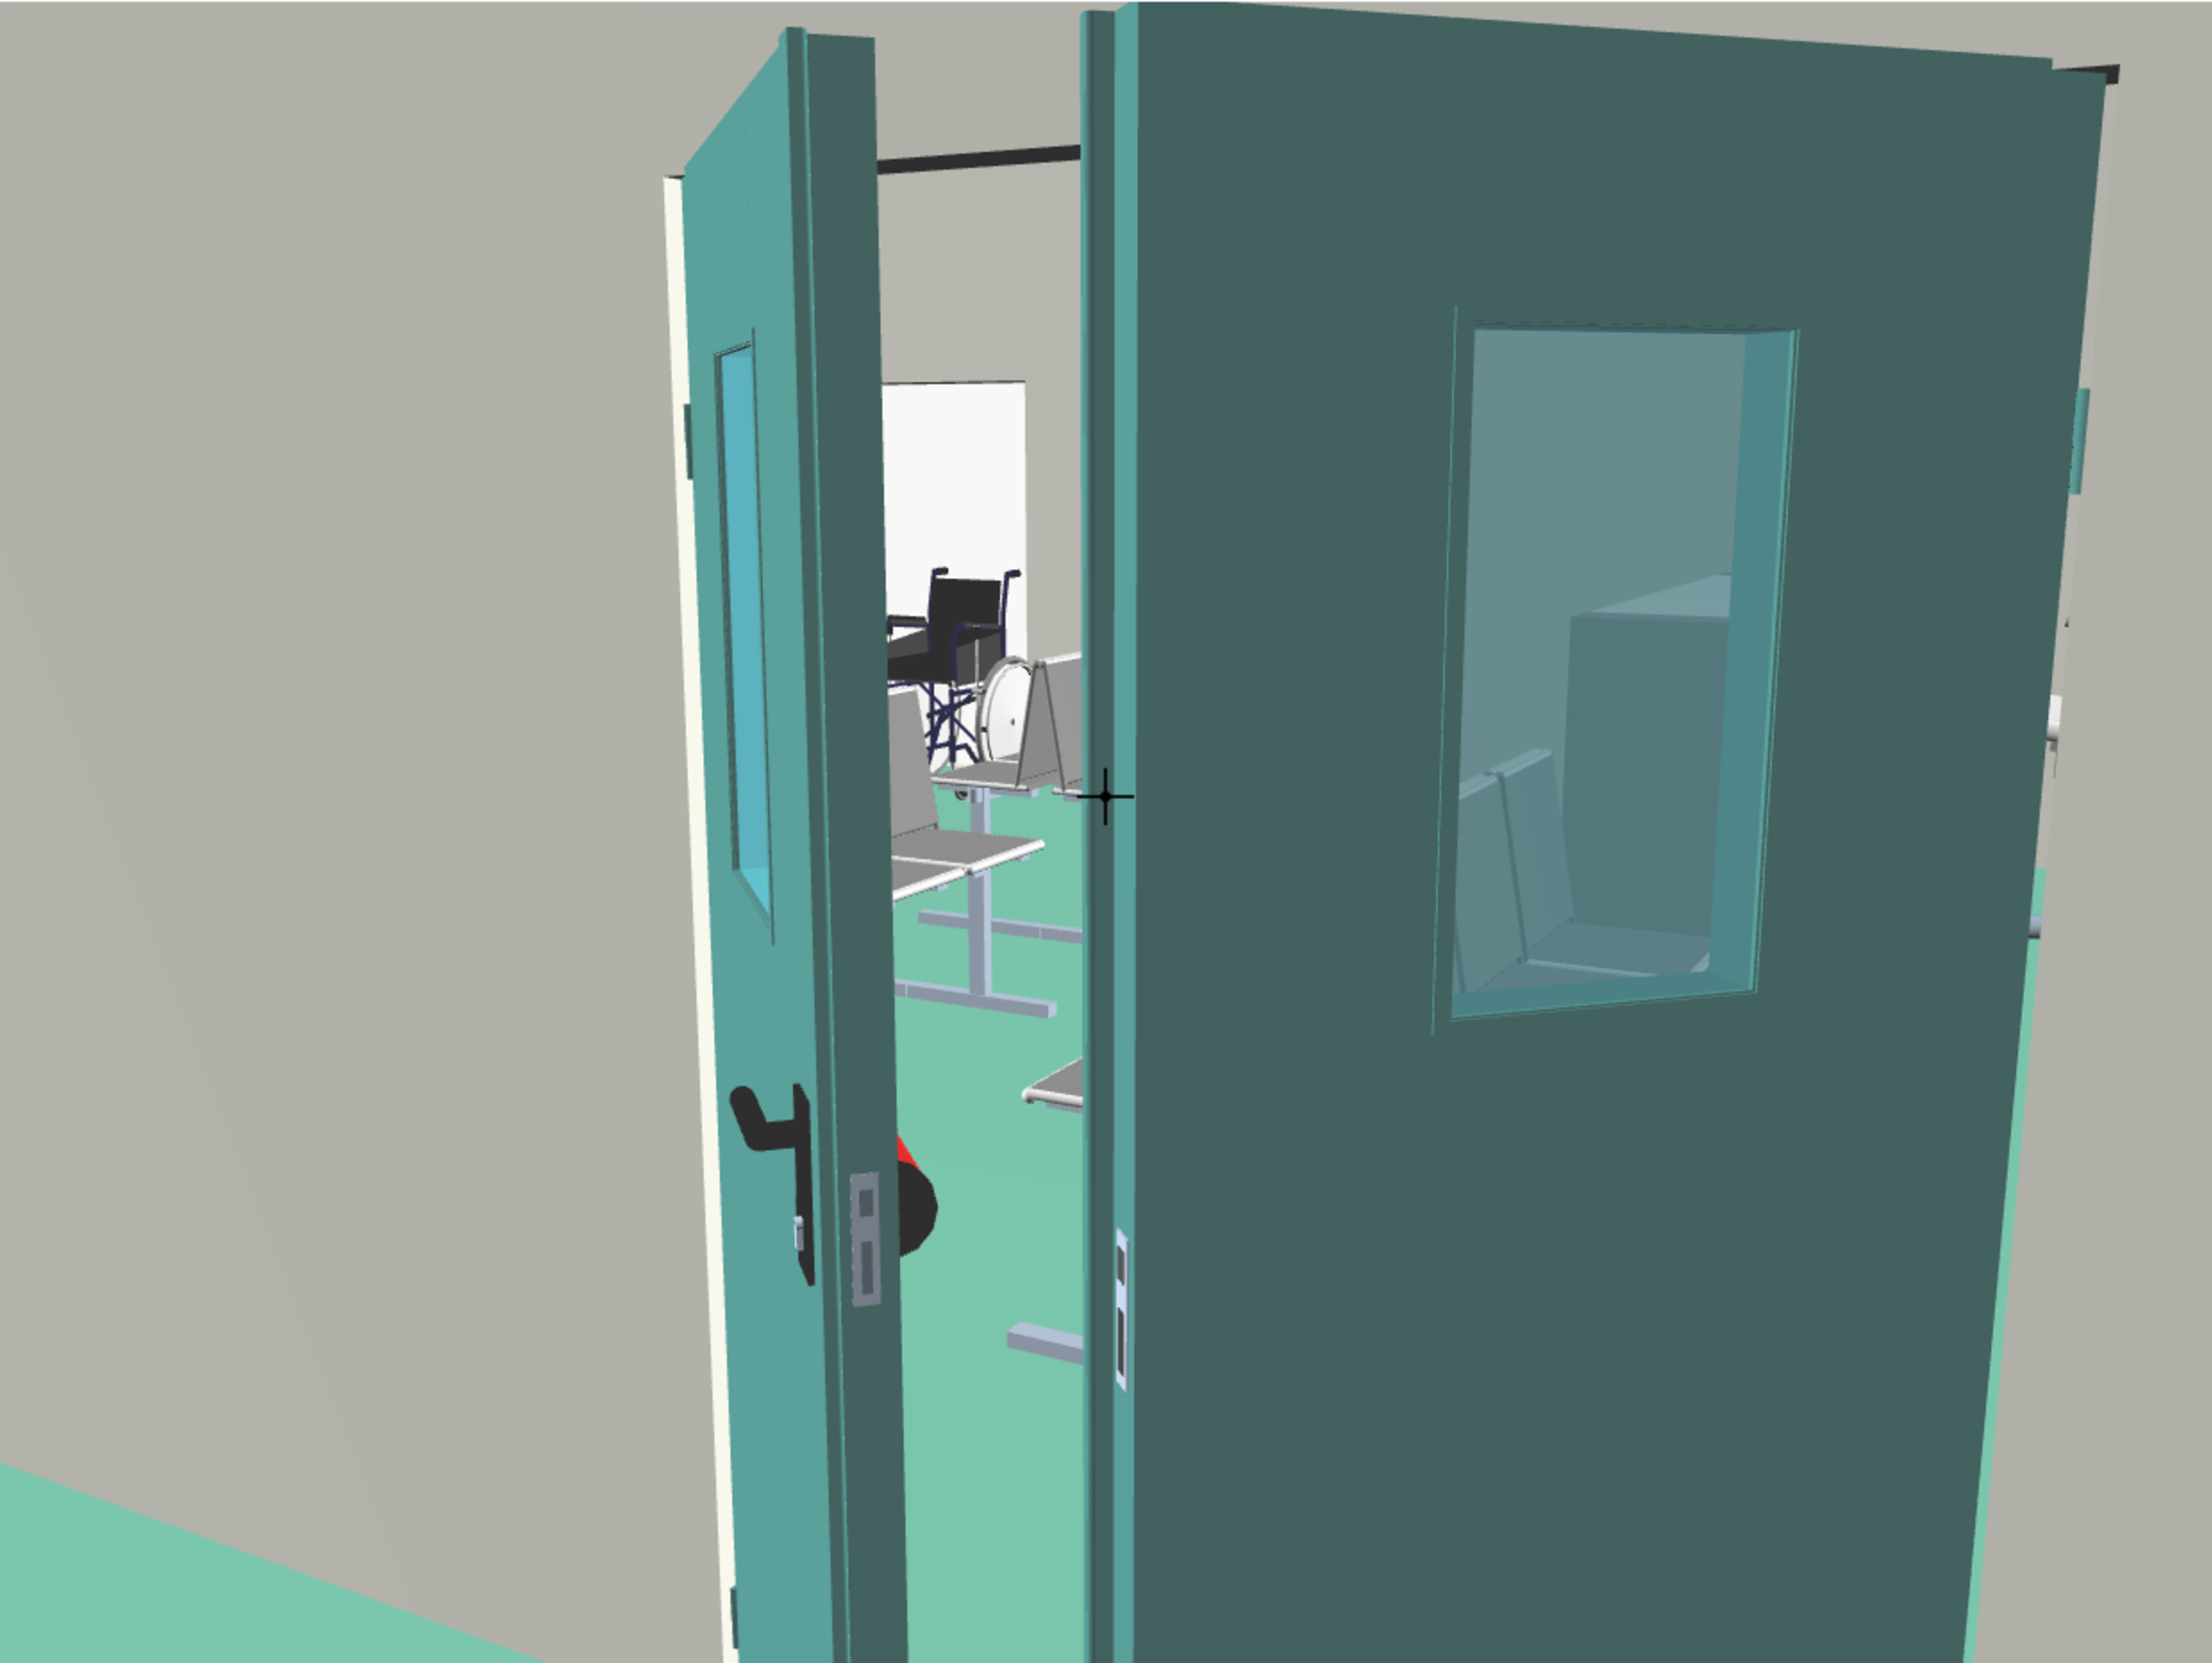
\includegraphics[width=\textwidth]{images/emergency/7}
   \caption{}
   \end{subfigure}
   
   \caption{LAR examples: (a) 2-chain of quad cells; (b) boundary 1-chain; (c) oriented boundary; (d) random 2-complex; (e) oriented 1-skeleton; (f) oriented boundary (in red).}
   \label{fig:meshes}
\end{figure*}


\end{document}

